\begin{table}
 \begin{tabular}{|C{15pt}|C{15pt}|C{15pt}|C{15pt}|C{15pt}|C{15pt}|C{15pt}|C{15pt}|C{15pt}|C{15pt}|C{15pt}|C{15pt}|C{15pt}|C{15pt}|C{15pt}|C{15pt}|C{15pt}|C{15pt}|}
  \multicolumn{18}{l}{(a) 1 layer with 18 elements}\\\hline
   0 & 1 & 2 & 3 & 4 & 5 & 6 & 7 & 8 & 9 & 10 & 11 & 12 & 13 & 14 & 15 & 16 & 17 \\\hline
  \multicolumn{18}{l}{}\\
  \multicolumn{18}{l}{(b) 2 layers with $11 + 10$ elements}\\\hline
   0 & 1 & 2 & 3 & 4 & 5 & 6 & 7 & 8 & 9 & \multicolumn{8}{c|}{$10 \le x$} \\\hline
   0 & \multicolumn{9}{c|}{$1 \le x \le 9$} & 10 & 11 & 12 & 13 & 14 & 15 & 16 & 17 \\\hline
  \multicolumn{18}{l}{}\\
  \multicolumn{18}{l}{(b) 3 layers with $9 + 9 + 6$ elements}\\\hline
   0 & 1 & 2 & 3 & 4 & 5 & 6 & 7 & \multicolumn{10}{c|}{$8 \le x$} \\\hline
   0 & \multicolumn{7}{c|}{$1 \le x \le 7$} & 8 & 9 & 10 & 11 & 12 & 13 & \multicolumn{4}{c|}{$14 \le x$}\\\hline
   0 & \multicolumn{13}{c|}{$1 \le x \le 13$} & 14 & 15 & 16 & 17 \\\hline
  \multicolumn{18}{l}{}\\
  \multicolumn{18}{l}{(b) 4 layers with $7 + 7 + 7 + 6$ elements}\\\hline
   0 & 1 & 2 & 3 & 4 & 5 & \multicolumn{12}{c|}{$6 \le x$} \\\hline
   0 & \multicolumn{5}{c|}{$1 \le x \le 5$} & 6 & 7 & 8 & 9 & \multicolumn{8}{c|}{$10 \le x$}\\\hline
   0 & \multicolumn{9}{c|}{$1 \le x \le 9$} & 10 & 11 & 12 & 13 & \multicolumn{4}{c|}{$14 \le x$}\\\hline
   0 & \multicolumn{13}{c|}{$1 \le x \le 13$} & 14 & 15 & 16 & 17 \\\hline
 \end{tabular}
\end{table}

\begin{table}
 \setlength{\doublerulesep}{.4pt}
\begin{tabular}{p{1.2cm}l@{~~}r}
  \hline\hline
  name & tuples & parameters \\\hline
\raisebox{10pt}{\begin{minipage}{1.2cm}
 \textsf{NT6-M}
 \mbox{1 layer}
\end{minipage}} &
\includegraphics[width=0.9cm]{figures/NTuple-0.pdf}
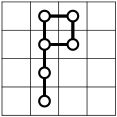
\includegraphics[width=0.9cm]{figures/NTuple-1.pdf}
\includegraphics[width=0.9cm]{figures/NTuple-2.pdf}
\includegraphics[width=0.9cm]{figures/NTuple-3.pdf}
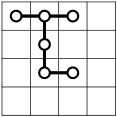
\includegraphics[width=0.9cm]{figures/NTuple-4.pdf}
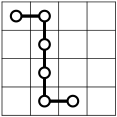
\includegraphics[width=0.9cm]{figures/NTuple-5.pdf}
\includegraphics[width=0.9cm]{figures/NTuple-6.pdf}
\includegraphics[width=0.9cm]{figures/NTuple-7.pdf}
& \raisebox{10pt}{$\begin{array}{r}
 % 18^6 \times 8 \times 1 \times 2\\
 18^6 \cdot 8 \cdot 1 \cdot 2\\
{}= 544\,195\,584
 \end{array}$}
\\\hline
\raisebox{10pt}{\begin{minipage}{1.2cm}
 \textsf{NT6}
 \mbox{1 layer}
\end{minipage}} & 
\includegraphics[width=0.9cm]{figures/NTuple-60.pdf}
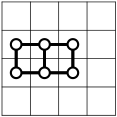
\includegraphics[width=0.9cm]{figures/NTuple-61.pdf}
\includegraphics[width=0.9cm]{figures/NTuple-62.pdf}
\includegraphics[width=0.9cm]{figures/NTuple-63.pdf}
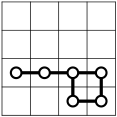
\includegraphics[width=0.9cm]{figures/NTuple-64.pdf}
\includegraphics[width=0.9cm]{figures/NTuple-65.pdf}
\includegraphics[width=0.9cm]{figures/NTuple-66.pdf}
\includegraphics[width=0.9cm]{figures/NTuple-67.pdf}
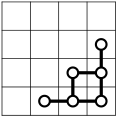
\includegraphics[width=0.9cm]{figures/NTuple-68.pdf}
& \raisebox{10pt}{$\begin{array}{r}
 % 18^6 \times 9 \times 1 \times 2\\
 18^6 \cdot 9 \cdot 1 \cdot 2\\
{}= 612\,220\,032
 \end{array}$}
\\\hline
\raisebox{10pt}{\begin{minipage}{1.2cm}
 \textsf{NT7}
 \mbox{2 layers}
\end{minipage}} &
\includegraphics[width=0.9cm]{figures/NTuple-70.pdf}
\includegraphics[width=0.9cm]{figures/NTuple-71.pdf}
\includegraphics[width=0.9cm]{figures/NTuple-72.pdf}
\includegraphics[width=0.9cm]{figures/NTuple-73.pdf}
\includegraphics[width=0.9cm]{figures/NTuple-74.pdf}
\includegraphics[width=0.9cm]{figures/NTuple-75.pdf}
\includegraphics[width=0.9cm]{figures/NTuple-76.pdf}

\includegraphics[width=0.9cm]{figures/NTuple-77.pdf}
& \raisebox{10pt}{$\begin{array}{r}
 % 11^7 \times 8 \times 2 \times 2\\
 11^7 \cdot 8 \cdot 2 \cdot 2\\
{}= 545\,640\,788
 \end{array}$}
\\\hline
\raisebox{10pt}{\begin{minipage}{1.2cm}
 \textsf{NT8}
 \mbox{3 layers}
\end{minipage}} &
\includegraphics[width=0.9cm]{figures/NTuple-80.pdf}
\includegraphics[width=0.9cm]{figures/NTuple-81.pdf}
\includegraphics[width=0.9cm]{figures/NTuple-82.pdf}
\includegraphics[width=0.9cm]{figures/NTuple-83.pdf}
\includegraphics[width=0.9cm]{figures/NTuple-84.pdf}
& \raisebox{10pt}{$\begin{array}{r}
 % 9^8 \times 5 \times 3 \times 2\\
 9^8 \cdot 5 \cdot 3 \cdot 2\\
{}= 1\,291\,401\,630
 \end{array}$}
\\\hline
\raisebox{10pt}{\begin{minipage}{1.2cm}
 \textsf{NT9}
 \mbox{4 layers}
\end{minipage}} &
\includegraphics[width=0.9cm]{figures/NTuple-90.pdf}
\includegraphics[width=0.9cm]{figures/NTuple-91.pdf}
\includegraphics[width=0.9cm]{figures/NTuple-92.pdf}
\includegraphics[width=0.9cm]{figures/NTuple-93.pdf}
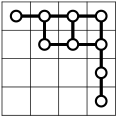
\includegraphics[width=0.9cm]{figures/NTuple-94.pdf}
\includegraphics[width=0.9cm]{figures/NTuple-95.pdf}
\includegraphics[width=0.9cm]{figures/NTuple-96.pdf}
& \raisebox{10pt}{$\begin{array}{r}
 % 7^9 \times 7 \times 4 \times 2\\
 7^9 \cdot 7 \cdot 4 \cdot 2\\
{}= 2\,259\,801\,992
 \end{array}$}
\\\hline
\end{tabular}
\end{table}

% 6G      NUM_TUPLES=8 NUM_SPLIT=1 で積は 48  メモリは  4.9GB (18^6*8*1*2*4*4)
% 6タプル NUM_TUPLES=9 NUM_SPLIT=1 で積は 54  メモリは  4.9GB (18^6*9*1*2*4*4)
% 7タプル NUM_TUPLES=7 NUM_SPLIT=2 で積は 98  メモリは  8.8GB (11^7*7*2*2*4*4)
% 8タプル NUM_TUPLES=5 NUM_SPLIT=3 で積は 120 メモリは 20.7GB ( 9^8*5*3*2*4*4)
% 9タプル NUM_TUPLES=7 NUM_SPLIT=4 で積は 252 メモリは 36.2GB ( 7^9*7*4*2*4*4)
